\clearpage % clear the prior chapter's page

\chapter{Supplement to "Methodology for rigorous modeling of protein conformational changes by Rosetta using DEER distance restraints"} \label{app:multilateration_supp}
%\vspace{-7mm}
%\bigskip

This Appendix contains supplementary information for Chapter \ref{ch:multilateration}.

%\vspace{-7mm}
%\bigskip

\begin{figure}[h]
\centering
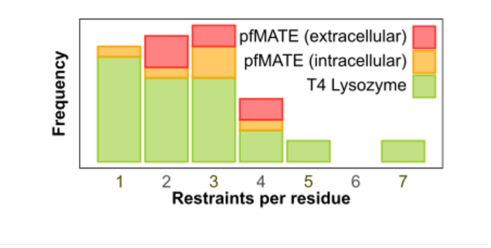
\includegraphics[width=2.5in]{Figures/multilateration_supp_n_restraints.pdf}
 \caption[Number of DEER restraints per spin-labeled residue across T4 Lysozyme and PfMATE.]{Number of DEER restraints per spin-labeled residue across T4 Lysozyme and PfMATE.}
\label{fig:multilateration_supp_n_restraints}
\end{figure}

\begin{figure}[h]
\centering
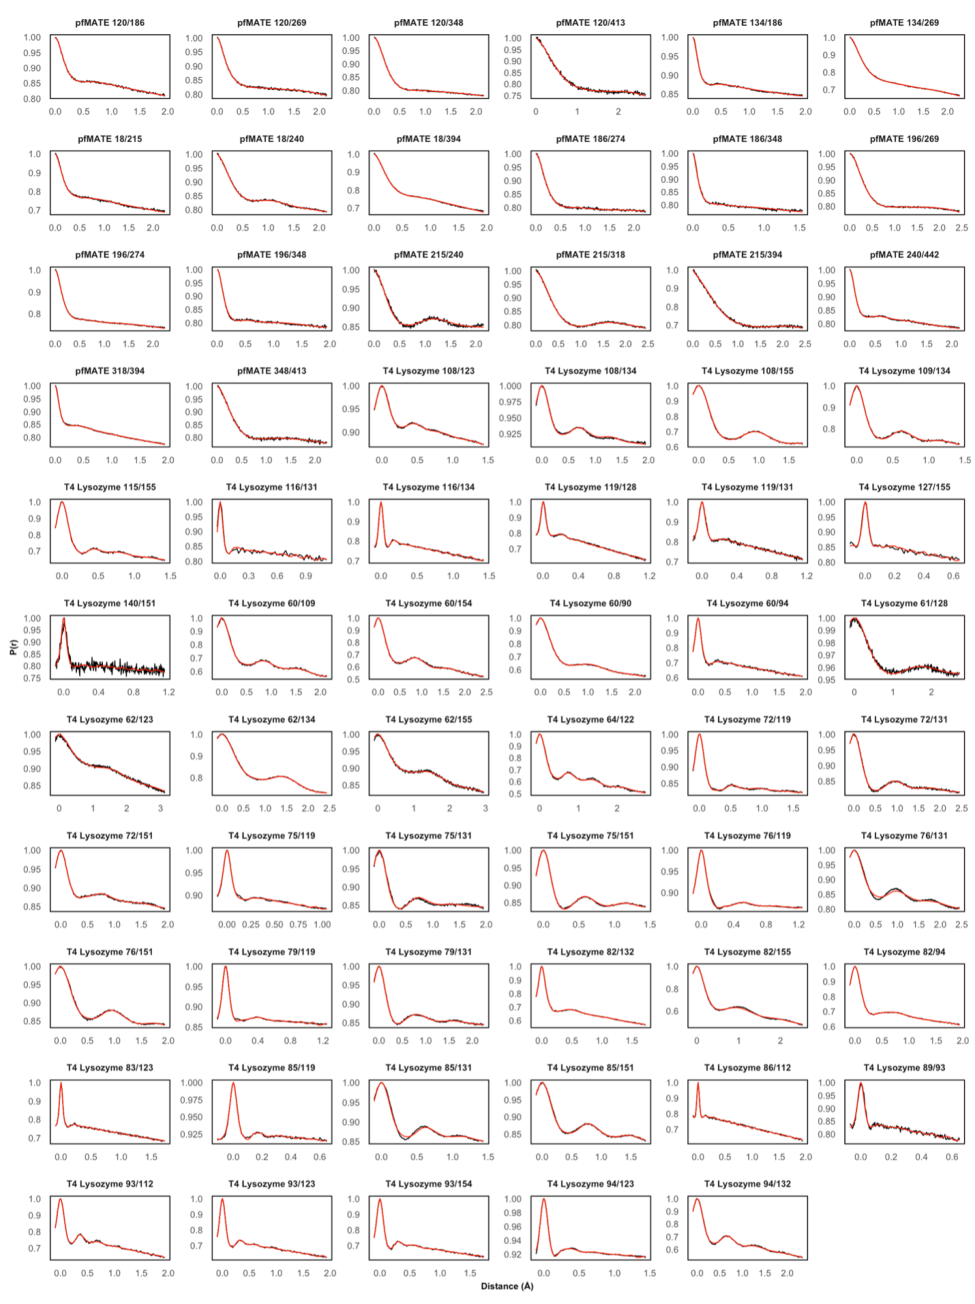
\includegraphics[width=6in]{Figures/multilateration_supp_alltraces.pdf}
\caption[All simulated and experimental DEER decay data used in this study between experimentally resolved residues.]{All simulated and experimental DEER decay data used in this study between experimentally resolved residues. All DEER traces determined by multilateration are shown in red. Experimental DEER traces are shown in black.}
\label{fig:multilateration_supp_alltraces}
\end{figure}

\begin{figure}[h]
\centering
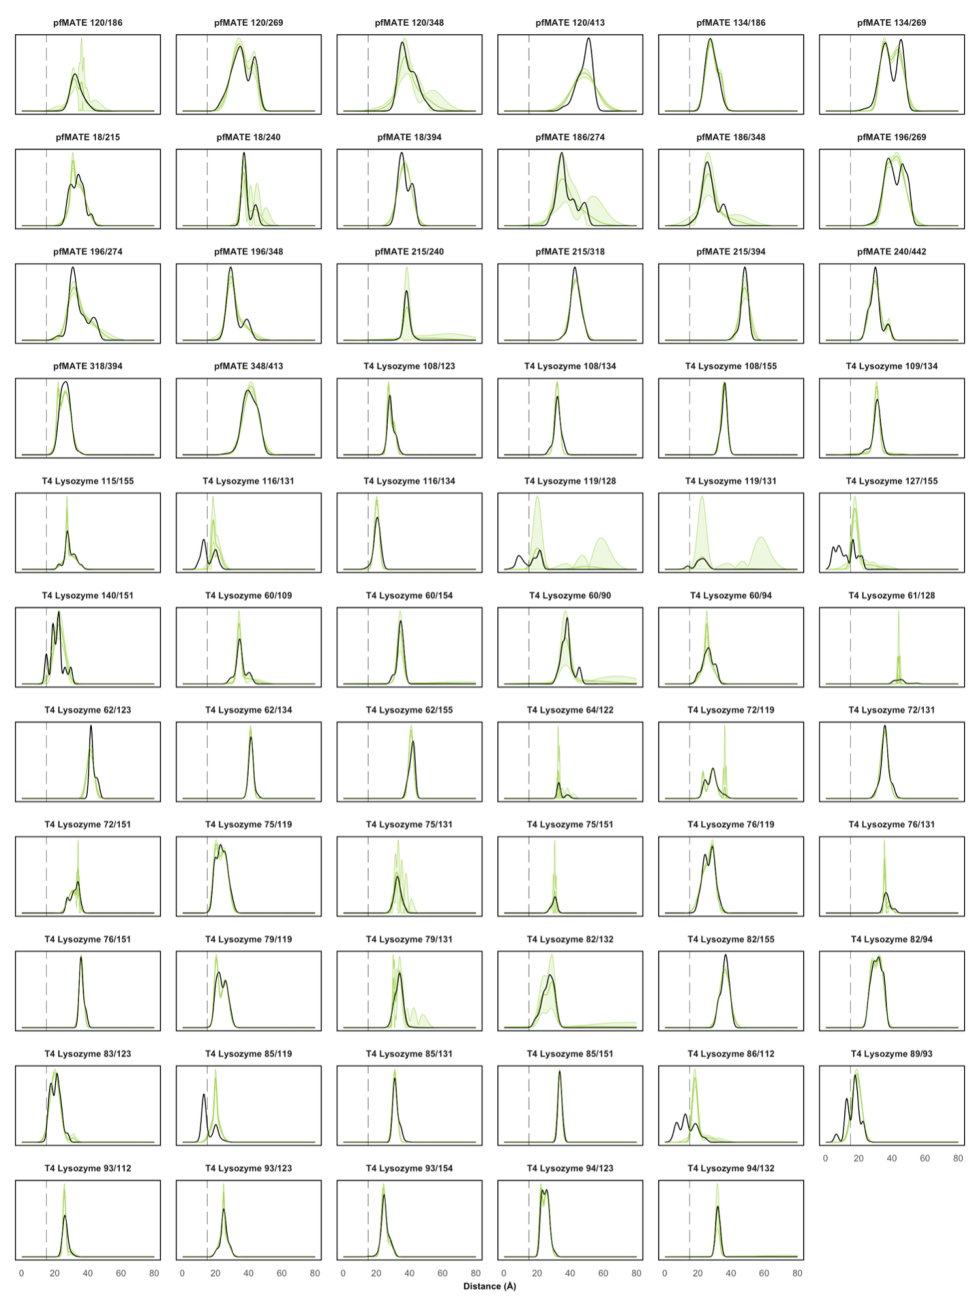
\includegraphics[width=6in]{Figures/multilateration_supp_gladdvu.pdf}
\caption[Comparison of distributions obtained using GLADDvu and those using the RosettaDEER multilateration algorithm.]{Comparison of distributions obtained using GLADDvu and those using the RosettaDEER multilateration algorithm. All DEER distance distributions determined by multilateration are shown in black. DEER distributions calculated using GladdVU are shown in green, with the shaded regions indicating 95\% confidence intervals. Distance values shorter than \SI{15}{\angstrom} (indicated by the dashed line) were not used to simulate DEER traces.}
\label{fig:multilateration_supp_gladdvu}
\end{figure}

\begin{figure}[h]
\centering
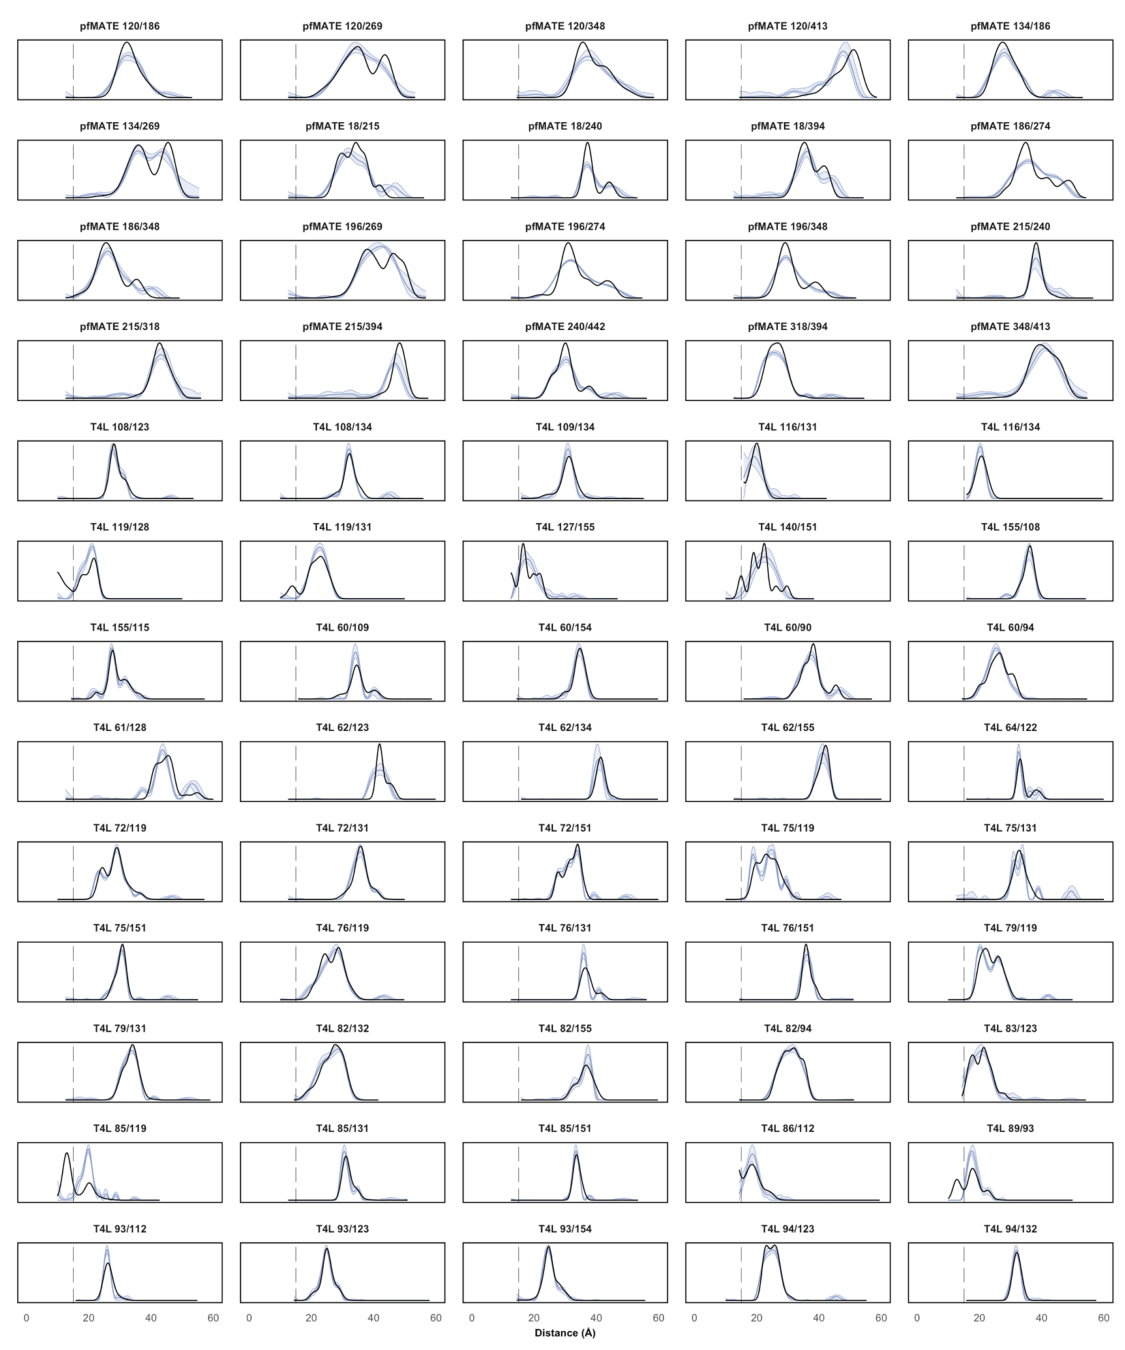
\includegraphics[width=6in]{Figures/multilateration_supp_deeranalysis.pdf}
\caption[Comparison of distributions obtained using DeerAnalysis and those using the RosettaDEER multilateration algorithm.]{Comparison of distributions obtained using DeerAnalysis and those using the RosettaDEER multilateration algorithm. All DEER distance distributions determined by multilateration are shown in black. DEER distributions calculated using DeerAnalysis are shown in green, with the shaded regions obtained using the validation tool.}
\label{fig:multilateration_supp_deeranalysis}
\end{figure}

\begin{figure}[h]
\centering
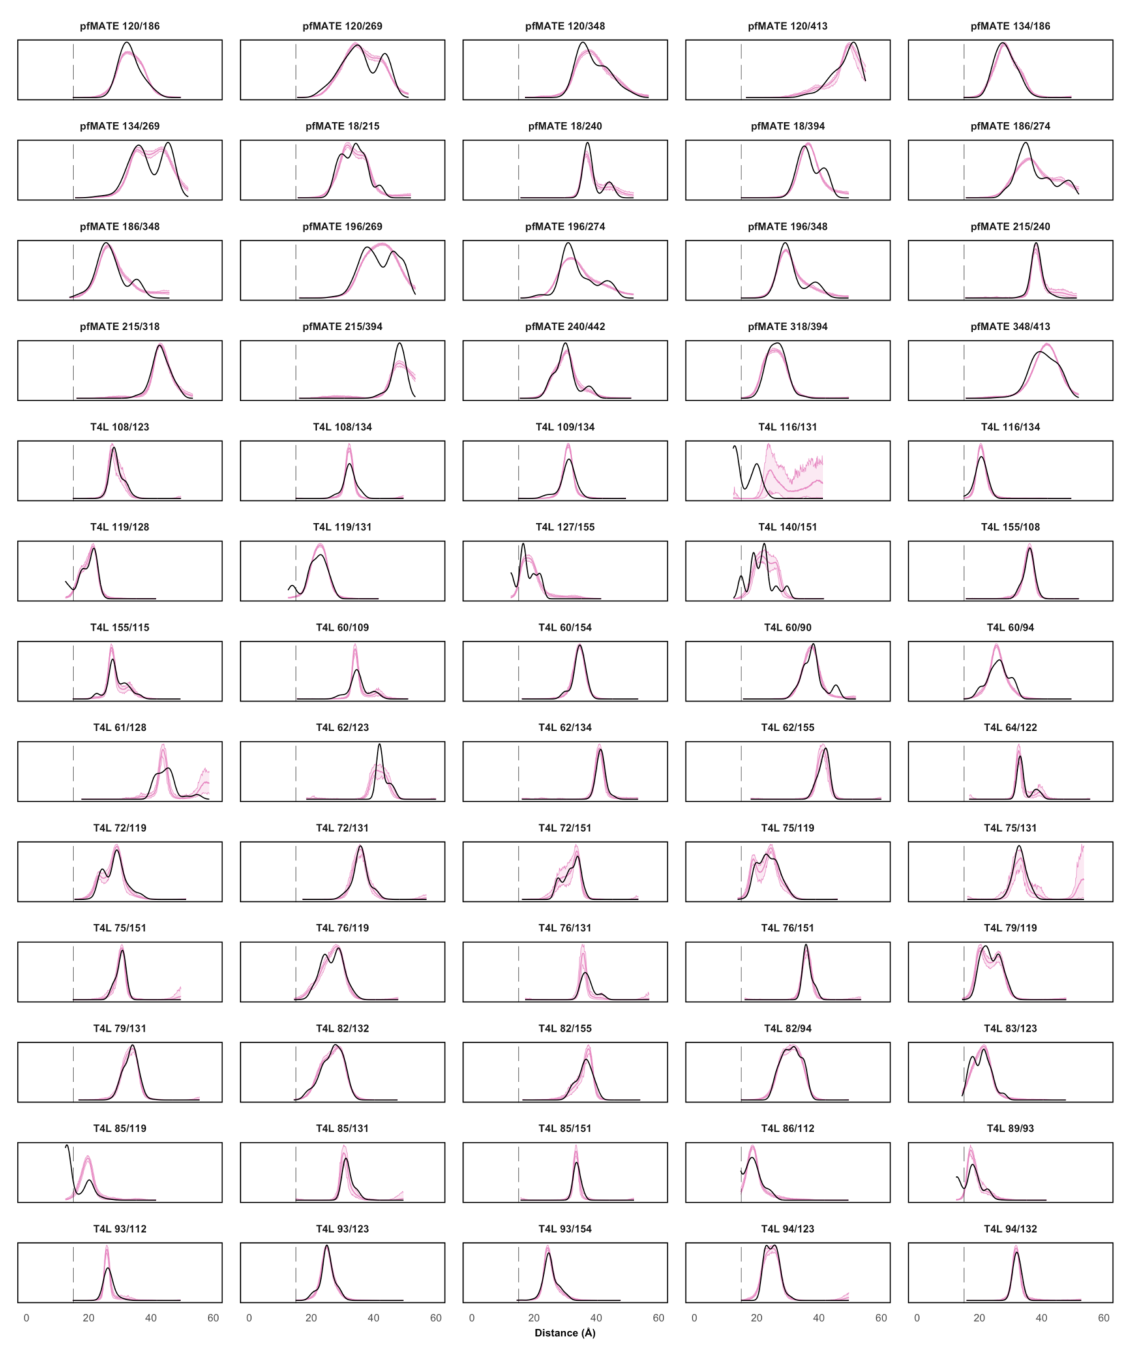
\includegraphics[width=6in]{Figures/multilateration_supp_deernet.pdf}
\caption[Comparison of distributions obtained using DeerNet and those using the RosettaDEER multilateration algorithm.]{Comparison of distributions obtained using DeerNet and those using the RosettaDEER multilateration algorithm. All DEER distance distributions determined by multilateration are shown in black. DEER distributions calculated using DeerNet are shown in pink, with the shaded regions obtained using ensemble statistics.}
\label{fig:multilateration_supp_deernet}
\end{figure}

\begin{figure}[h]
\centering
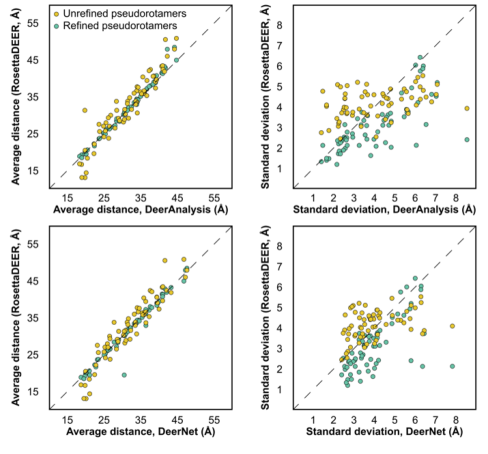
\includegraphics[width=3.5in]{Figures/multilateration_supp_avgs_stdevs.pdf}
\caption[Comparison of average and standard deviation values obtained when fitting DEER data collected in pfMATE and T4 Lysozyme to values obtained using DeerAnalysis and DeerNet.]{Comparison of average and standard deviation values obtained when fitting DEER data collected in pfMATE and T4 Lysozyme to values obtained using DeerAnalysis and DeerNet. Long-distance fitting artifacts were removed from fits obtained using DeerAnalysis. These fits appeared to overstate the standard deviation values relative to GLADDvu, whereas those obtained using DeerNet appeared to be biased toward certain width values.}
\label{fig:multilateration_supp_avgs_stdev}
\end{figure}

\begin{figure}[h]
\centering
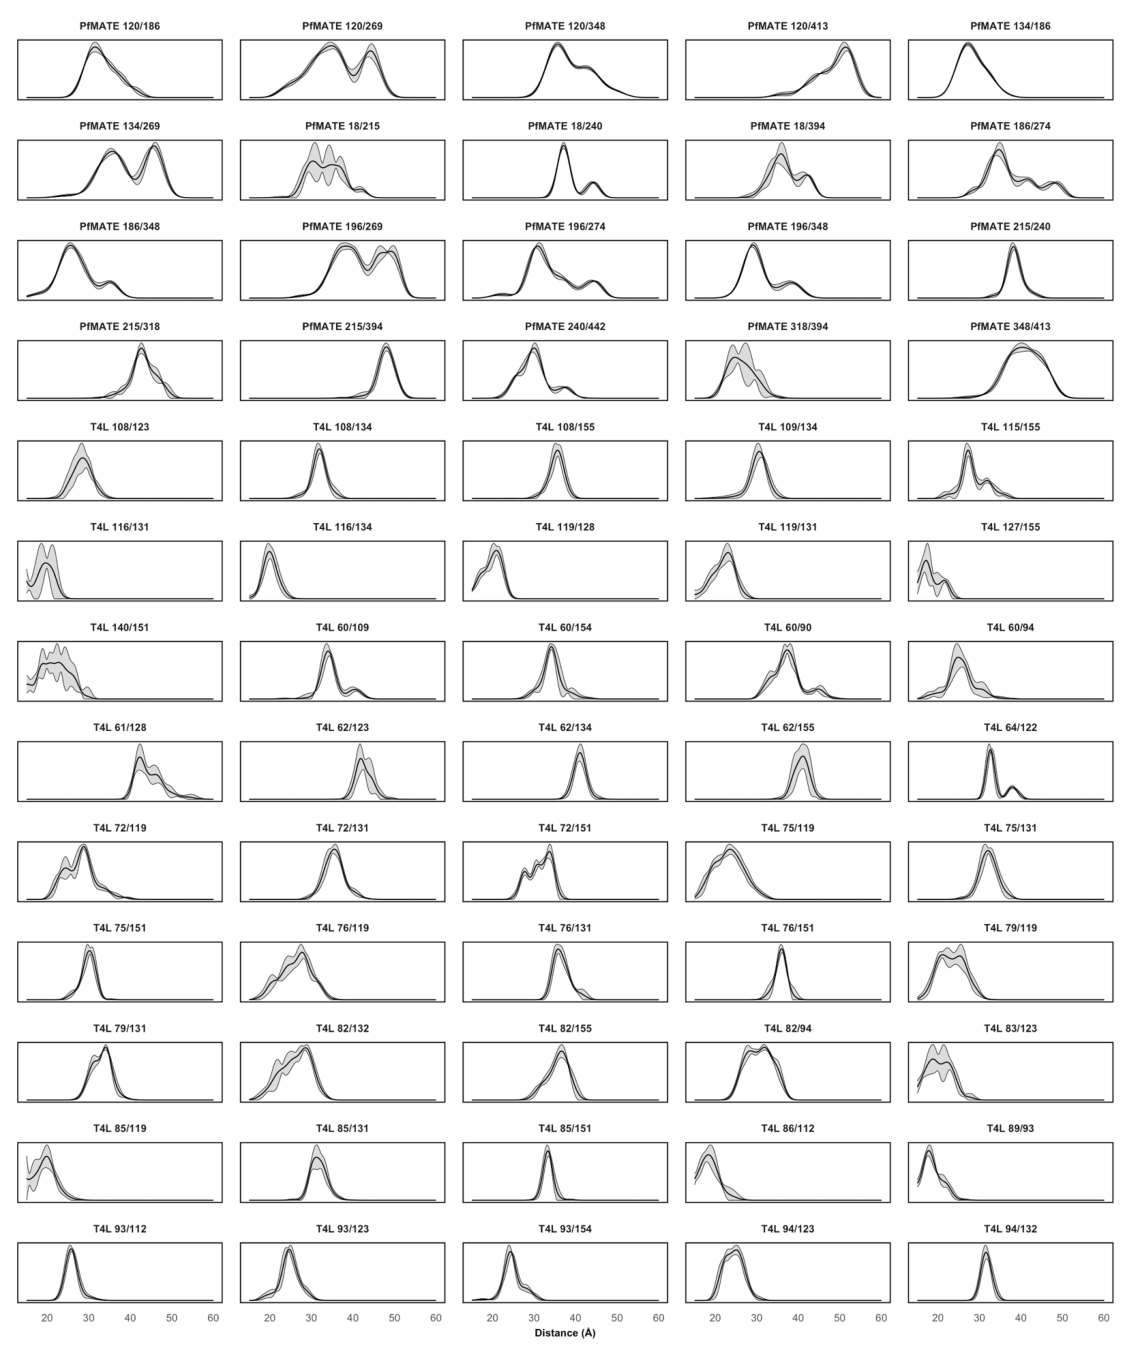
\includegraphics[width=6in]{Figures/multilateration_supp_conf_bands.pdf}
\caption[Confidence analysis among the five best-scoring rotamer ensembles generated using the RosettaDEER multilateration algorithm. ]{Confidence analysis among the five best-scoring rotamer ensembles generated using the RosettaDEER multilateration algorithm. Shaded regions depict 95\% confidence intervals, and line represents the mean distribution. Ensembles were selected using the \gls{aicc}.}
\label{fig:multilateration_supp_conf_bands}
\end{figure}

\begin{figure}[h]
\centering
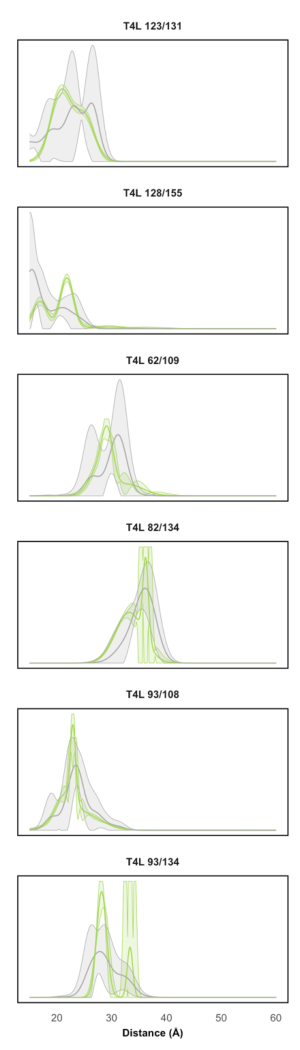
\includegraphics[width=2.in]{Figures/multilateration_supp_validation.pdf}
\caption[Comparison of DEER distance distributions used to validate pseudo-rotamers obtained using the RosettaDEER multilateration algorithm.]{Comparison of DEER distance distributions used to validate pseudo-rotamers obtained using the RosettaDEER multilateration algorithm. Distributions obtained using GLADDvu and RosettaDEER are shown in green and grey, respectively. Confidence bands for RosettaDEER depict the five best sets of pseudo-rotamers.}
\label{fig:multilateration_supp_validation}
\end{figure}

\begin{figure}[h]
\centering
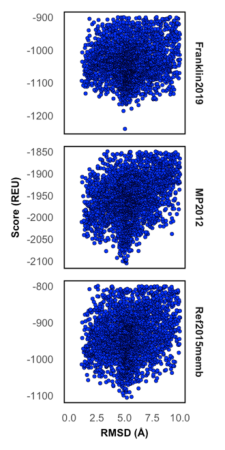
\includegraphics[width=2in]{Figures/multilateration_supp_scores.pdf}
\caption[Rosetta energy functions for membrane proteins cannot identify the inward-facing conformation of PfMATE.]{Rosetta energy functions for membrane proteins cannot identify the inward-facing conformation of PfMATE.  In all three cases, the lowest-energy models are fully occluded from both sides of the membrane. RMSD is measured from the inward-facing crystal structure (PDB: 6FHZ); the first 50 residues were omitted.}
\label{fig:multilateration_supp_scores}
\end{figure}